\documentclass[journal,12pt,twocolumn]{IEEEtran}
\usepackage{setspace}
\usepackage{gensymb}
\usepackage{iithtlc}
%\usepackage{xcolor}
\usepackage{caption}
\usepackage{fullpage}
\usepackage[american]{circuitikz}
\usetikzlibrary{circuits.logic.US}
\usepackage{circuitikz}
\usetikzlibrary{positioning}
\usetikzlibrary{matrix,calc}
%\usepackage{subcaption}
%\doublespacing
\singlespacing

%\usepackage{graphicx}
%\usepackage{amssymb}
%\usepackage{relsize}
\usepackage[cmex10]{amsmath}
\usepackage{mathtools}
%\usepackage{amsthm}
%\interdisplaylinepenalty=2500
%\savesymbol{iint}
%\usepackage{txfonts}
%\restoresymbol{TXF}{iint}
%\usepackage{wasysym}
\usepackage{amsthm}
\usepackage{mathrsfs}
\usepackage{txfonts}
\usepackage{stfloats}
\usepackage{cite}
\usepackage{cases}
\usepackage{subfig}
%\usepackage{xtab}
\usepackage{longtable}
\usepackage{multirow}
%\usepackage{algorithm}
%\usepackage{algpseudocode}
%\usepackage{enumitem}
\usepackage{enumerate}
\usepackage{mathtools}
\usepackage{multicol}

\usepackage[framemethod=tikz]{mdframed}

%\usepackage{listings}
%\usepackage{listings}
%    \usepackage[latin1]{inputenc}                                 %%
%    \usepackage{color}                                            %%
%    \usepackage{array}                                            %%
%    \usepackage{longtable}                                        %%
%    \usepackage{calc}                                             %%
%    \usepackage{multirow}                                         %%
    \usepackage{hhline}                                           %%
    \usepackage{ifthen}                                           %%
  %optionally (for landscape tables embedded in another document): %%
    \usepackage{lscape}     
\usepackage{tikz}


%\usepackage{stmaryrd}


%\usepackage{wasysym}
%\newcounter{MYtempeqncnt}
\DeclareMathOperator*{\Res}{Res}
%\renewcommand{\baselinestretch}{2}
\renewcommand\thesection{\arabic{section}}
\renewcommand\thesubsection{\thesection.\arabic{subsection}}
\renewcommand\thesubsubsection{\thesubsection.\arabic{subsubsection}}

\renewcommand\thesectiondis{\arabic{section}}
\renewcommand\thesubsectiondis{\thesectiondis.\arabic{subsection}}
\renewcommand\thesubsubsectiondis{\thesubsectiondis.\arabic{subsubsection}}

% correct bad hyphenation here
\hyphenation{op-tical net-works semi-conduc-tor}

%\lstset{
%language=C,
%frame=single, 
%breaklines=true
%}

%\lstset{
	%%basicstyle=\small\ttfamily\bfseries,
	%%numberstyle=\small\ttfamily,
	%language=Octave,
	%backgroundcolor=\color{white},
	%%frame=single,
	%%keywordstyle=\bfseries,
	%%breaklines=true,
	%%showstringspaces=false,
	%%xleftmargin=-10mm,
	%%aboveskip=-1mm,
	%%belowskip=0mm
%}

%\surroundwithmdframed[width=\columnwidth]{./figs/lstlisting}
%\def\inputGnumericTable{}                                 %%

%\lstset{
%language=C,
%frame=single, 
%breaklines=true
%}
%\lstset{
%language=assembly,
%frame=single, 
%breaklines=true
%}
 

\begin{document}
%

\theoremstyle{definition}
\newtheorem{theorem}{Theorem}[section]
\newtheorem{problem}{Problem}
\newtheorem{proposition}{Proposition}[section]
\newtheorem{lemma}{Lemma}[section]
\newtheorem{corollary}[theorem]{Corollary}
\newtheorem{example}{Example}[section]
\newtheorem{definition}{Definition}[section]
%\newtheorem{algorithm}{Algorithm}[section]
%\newtheorem{cor}{Corollary}
\newcommand{\BEQA}{\begin{eqnarray}}
\newcommand{\EEQA}{\end{eqnarray}}
\newcommand{\define}{\stackrel{\triangle}{=}}

\bibliographystyle{IEEEtran}
%\bibliographystyle{ieeetr}

\providecommand{\nCr}[2]{\,^{#1}C_{#2}} % nCr
\providecommand{\nPr}[2]{\,^{#1}P_{#2}} % nPr
\providecommand{\mbf}{\mathbf}
\providecommand{\pr}[1]{\ensuremath{\Pr\left(#1\right)}}
\providecommand{\qfunc}[1]{\ensuremath{Q\left(#1\right)}}
\providecommand{\sbrak}[1]{\ensuremath{{}\left[#1\right]}}
\providecommand{\lsbrak}[1]{\ensuremath{{}\left[#1\right.}}
\providecommand{\rsbrak}[1]{\ensuremath{{}\left.#1\right]}}
\providecommand{\brak}[1]{\ensuremath{\left(#1\right)}}
\providecommand{\lbrak}[1]{\ensuremath{\left(#1\right.}}
\providecommand{\rbrak}[1]{\ensuremath{\left.#1\right)}}
\providecommand{\cbrak}[1]{\ensuremath{\left\{#1\right\}}}
\providecommand{\lcbrak}[1]{\ensuremath{\left\{#1\right.}}
\providecommand{\rcbrak}[1]{\ensuremath{\left.#1\right\}}}
\theoremstyle{remark}
\newtheorem{rem}{Remark}
\newcommand{\sgn}{\mathop{\mathrm{sgn}}}
\providecommand{\abs}[1]{\left\vert#1\right\vert}
\providecommand{\res}[1]{\Res\displaylimits_{#1}} 
\providecommand{\norm}[1]{\lVert#1\rVert}
\providecommand{\mtx}[1]{\mathbf{#1}}
\providecommand{\mean}[1]{E\left[ #1 \right]}
\providecommand{\fourier}{\overset{\mathcal{F}}{ \rightleftharpoons}}
%\providecommand{\hilbert}{\overset{\mathcal{H}}{ \rightleftharpoons}}
\providecommand{\system}{\overset{\mathcal{H}}{ \longleftrightarrow}}
	%\newcommand{\solution}[2]{\textbf{Solution:}{#1}}
\newcommand{\solution}{\noindent \textbf{Solution: }}
\providecommand{\dec}[2]{\ensuremath{\overset{#1}{\underset{#2}{\gtrless}}}}
%\numberwithin{equation}{subsection}
\numberwithin{equation}{problem}
%\numberwithin{problem}{subsection}
%\numberwithin{definition}{subsection}
%\makeatletter
%\@addtoreset{figure}{problem}
%\makeatother
%
%\let\StandardTheFigure\thefigure
%%\renewcommand{\thefigure}{\theproblem.\arabic{figure}}
%\renewcommand{\thefigure}{\theproblem}
%

%\numberwithin{figure}{subsection}

%\numberwithin{equation}{subsection}
%\numberwithin{equation}{section}
%%\numberwithin{equation}{problem}
%%\numberwithin{problem}{subsection}
\numberwithin{problem}{section}
%%\numberwithin{definition}{subsection}
%\makeatletter
%\@addtoreset{figure}{problem}
%\makeatother
\makeatletter
\@addtoreset{table}{problem}
\makeatother

\let\StandardTheFigure\thefigure
\let\StandardTheTable\thetable
%%\renewcommand{\thefigure}{\theproblem.\arabic{figure}}
%\renewcommand{\thefigure}{\theproblem}
\renewcommand{\thetable}{\theproblem}
%%\numberwithin{figure}{section}

%%\numberwithin{figure}{subsection}

\renewcommand{\thefigure}{\theenumi}

\def\putbox#1#2#3{\makebox[0in][l]{\makebox[#1][l]{}\raisebox{\baselineskip}[0in][0in]{\raisebox{#2}[0in][0in]{#3}}}}
     \def\rightbox#1{\makebox[0in][r]{#1}}
     \def\centbox#1{\makebox[0in]{#1}}
     \def\topbox#1{\raisebox{-\baselineskip}[0in][0in]{#1}}
     \def\midbox#1{\raisebox{-0.5\baselineskip}[0in][0in]{#1}}

\vspace{3cm}

\title{ 
	\logo{
GATE Exercises on Digital Design
	}
}



% paper title
% can use linebreaks \\ within to get better formatting as desired
%\title{Matrix Analysis through Octave}
%
%
% author names and IEEE memberships
% note positions of commas and nonbreaking spaces ( ~ ) LaTeX will not break
% a structure at a ~ so this keeps an author's name from being broken across
% two lines.
% use \thanks{} to gain access to the first footnote area
% a separate \thanks must be used for each paragraph as LaTeX2e's \thanks
% was not built to handle multiple paragraphs
%

%\author{G V V Sharma$^{*}$% <-this % stops a space
%\thanks{*The author is with the Department
%of Electrical Engineering, Indian Institute of Technology, Hyderabad
%502285 India e-mail:  gadepall@iith.ac.in.}% <-this % stops a space
%%\thanks{J. Doe and J. Doe are with Anonymous University.}% <-this % stops a space
%%\thanks{Manuscript received April 19, 2005; revised January 11, 2007.}}
%}
% note the % following the last \IEEEmembership and also \thanks - 
% these prevent an unwanted space from occurring between the last author name
% and the end of the author line. i.e., if you had this:
% 
% \author{....lastname \thanks{...} \thanks{...} }
%                     ^------------^------------^----Do not want these spaces!
%
% a space would be appended to the last name and could cause every name on that
% line to be shifted left slightly. This is one of those "LaTeX things". For
% instance, "\textbf{A} \textbf{B}" will typeset as "A B" not "AB". To get
% "AB" then you have to do: "\textbf{A}\textbf{B}"
% \thanks is no different in this regard, so shield the last } of each \thanks
% that ends a line with a % and do not let a space in before the next \thanks.
% Spaces after \IEEEmembership other than the last one are OK (and needed) as
% you are supposed to have spaces between the names. For what it is worth,
% this is a minor point as most people would not even notice if the said evil
% space somehow managed to creep in.



% The paper headers
%\markboth{Journal of \LaTeX\ Class Files,~Vol.~6, No.~1, January~2007}%
%{Shell \MakeLowercase{\textit{et al.}}: Bare Demo of IEEEtran.cls for Journals}
% The only time the second header will appear is for the odd numbered pages
% after the title page when using the twoside option.
% 
% *** Note that you probably will NOT want to include the author's ***
% *** name in the headers of peer review papers.                   ***
% You can use \ifCLASSOPTIONpeerreview for conditional compilation here if
% you desire.




% If you want to put a publisher's ID mark on the page you can do it like
% this:
%\IEEEpubid{0000--0000/00\$00.00~\copyright~2007 IEEE}
% Remember, if you use this you must call \IEEEpubidadjcol in the second
% column for its text to clear the IEEEpubid mark.



% make the title area
\maketitle

%\tableofcontents

\bigskip

\begin{abstract}
%\boldmath
This problem set has questions related to combinational and sequential circuits taken from GATE papers over the last twenty years.  Teachers can use the problem set for courses tutorials. 
 
\end{abstract}

\begin{enumerate}
\item Convert an $S-R$ FLIP-FLOP into a $T$ FLIP FLOP.



\item A sequential multiplexer is connected as shown in Fig. \ref{fig:1}. Each time the multiplexer receives the clock, it switches to the next channel(From $6$ it goes to $1$). If the input signals are


\begin{enumerate}[(a)]
 
\item $
A = 5 \cos 2 \pi (4 \times 10^3 t)
$

\item $
B = 2 \cos 2 \pi (3.8 \times 10^3 t)
$

\item $
C = 6 \cos 2 \pi (2.2 \times 10^3 t)
$

\item $
D = 4 \cos 2 \pi (1.7 \times 10^3 t)
$


\end{enumerate}

\begin{figure}

\centering

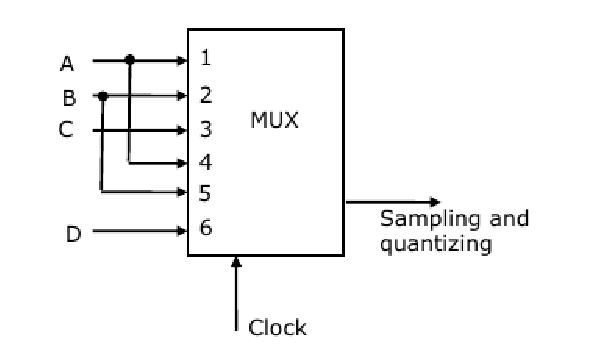
\includegraphics[width=\columnwidth]{./figs/1.eps}

\caption{}

\label{fig:1}

\end{figure} 




 the minimum clock frequency should be $ \rule{3cm}{0.15mm}$ $KHz$.
 
 
\item The logic realized by the circuit shown in Fig. \ref{fig:2} is :



\begin{figure}

\centering

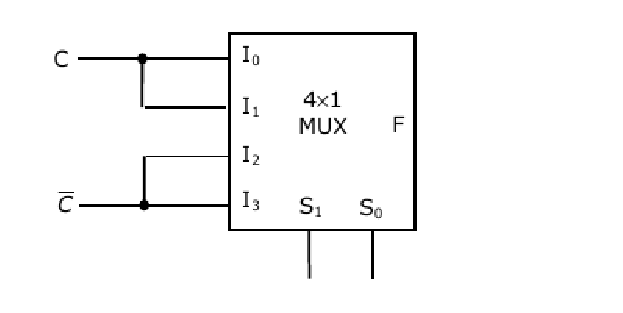
\includegraphics[width=\columnwidth]{./figs/2.eps}

\caption{}

\label{fig:2}

\end{figure} 



\begin{enumerate}[(a)]
 
\item $
F = A.C
$

\item $
F = A + C
$

\item $
F = B.C
$

\item $
F = B + C
$


\end{enumerate}


\item The initial contents of the $4 -$bit serial-in-parallel-out, right-shift, Shift Register shown in Fig. \ref{fig:3} , is $ 0 \ 1 \ 1 \ 0 $. After three clock pulses are applied, the contents of the Shift Register will be

\begin{figure}

\centering

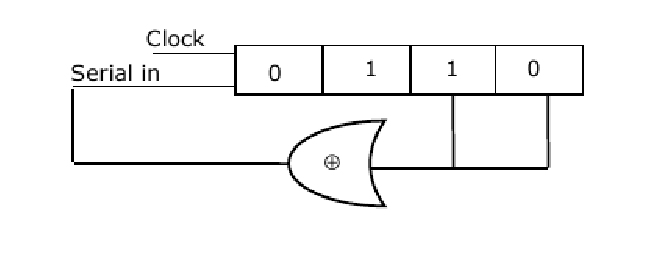
\includegraphics[width=\columnwidth]{./figs/3.eps}

\caption{}

\label{fig:3}

\end{figure} 


\begin{enumerate}[(a)]
 
\item $
0 \ 0 \ 0 \ 0
$

\item $
0 \ 1 \ 0 \ 1
$

\item $
1 \ 0 \ 1 \ 0
$

\item $
1 \ 1 \ 1 \ 1
$


\end{enumerate}


\item A new clocked $X-Y$ flip flop is defined with two inputs, $X$ and $Y$ is addition to the clock input. The flip flop functions as follows:

If $XY=00$, the flip flop changes stage with each clock pulse

If $XY=01$, the flip flop state Q becomes $1$ with the next clock pulse

If $XY=10$, the flip flop state Q becomes $0$ with the next clock pulse

If $XY=11$, the change of state occurs with the clock pulse

\begin{enumerate}[(a)]
 
\item Write the Truth table for the $X-Y$ flip flop

\item Write the Excitation table for the $X-Y$ flip flop

\item It is desired to convert a $J-K$ flip flop into the $X-Y$ flip flop by adding some external gates, if necessary. Draw a circuit to show how you will implement in $X-Y$ flip flop using a $J-K$ flip flop.


\end{enumerate}

\item $2$'s complement representation of a $16$-bit number (one sign bit and $15$ magnitude bits) is FFFI. Its magnitude in decimal representation is


\begin{enumerate}[(a)]
 
\item $
0
$

\item $
1
$

\item $
32,767
$

\item $
65, 535
$


\end{enumerate}

\item Signals $A,B,C,D$ and $\bar{D}$ are available. Using a single $8$ to $1$ multiplexer and no other gate, implement the Boolean function $f(A,B,C,D)=B.C + A.B.\bar{D} + \bar{A}.\bar{C}.D$


\item A clocked sequential circuit has three states, $A$, $B$ and $C$ and one input $X$. As long as the input $X$ is $0$, the circuit alternates between the states $A$ and $B$. If the input $X$ becomes $1$ ( either in state $A$ or in state $B$),the circuit goes to state $C$ and remains in state $C$ as long as $X$ continues to be $1$. The circuit returns to state $A$ if the input becomes $0$ once again and from then on repeats its behaviour.Assume that the state assignments are $A=00$, $B=01$ and $C=10$.

\begin{enumerate}[(a)]
 
\item Draw the state diagram of the circuit

\item Give the state table for the circuit

\item Draw the circuit using $D$ flip flops
\end{enumerate}

\item Match each of the items $A$,$B$ and $C$ with an appropriate item on the right. 

\begin{enumerate}[(a)]

\begin{multicols}{2}
 
\item A shift register can be used

\item A multiplexer can be used

\item A decoder can be used


\columnbreak

(1) for code conversion

(2) to generate memory chip select

(3) for parallel-to-serial conversion

(4) as a many-to-one switch

(5) for analog-to-digital conversion


\end{multicols}
\end{enumerate}






\item A $2$ bit binary multiplier can be implemented using

\begin{enumerate}[(a)]
 
\item $2$ inputs ANDs only

\item $2$ input XORs and $4$ input AND gates only

\item Two $2$ inputs NORs and one XNOR gate

\item XOR gates and shift registers


\end{enumerate}

\item A signed integer has been stored in a byte using the $2$'s complement format. We wish to store the same integer in a $16$ bit word. We should
\begin{enumerate}[(a)]
 
\item copy the original byte to the less significant byte of the word and fill the more significant with zeros

\item copy the original byte to the more significant byte of the word and fill the less significant byte with zeros

\item copy the original byte to the less significant byte of the word and make each fit of the more significant byte equal to the most significant bit of the original byte

\item copy the original byte to the less significant byte as well as the more significant byte of the word

\end{enumerate}

\item In a $J-K$ flip-flop we have $J=Q$ and $K=1$. Assuming the flip flop was initially cleared and then clocked for $6$ pulses, the sequence at the $Q$ output will be

\begin{figure}

\centering

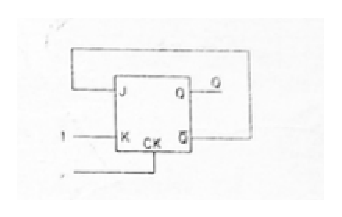
\includegraphics[width=\columnwidth]{./figs/4.eps}

\caption{}

\label{fig:4}

\end{figure} 

 
 
\begin{enumerate}[(a)]

\item $
010000
$

\item $
011001
$

\item $
010010
$

\item $
010101
$

\end{enumerate}

\item A sequence generator is shown in the Fig. \ref{fig:5} is 
The counter status $(Q_0,Q_1,Q_2)$ is initialised to $010$ using preset/clear inputs.

\begin{figure}

\centering

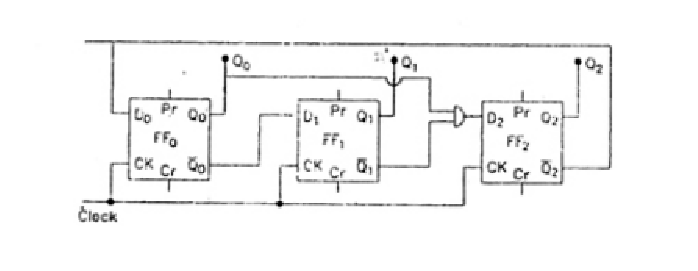
\includegraphics[width=\columnwidth]{./figs/5.eps}

\caption{}

\label{fig:5}

\end{figure} 


The clock has a period of $50$ ns and transitions take place at the rising clock edge.


\begin{enumerate}[(a)]
 
\item Give the sequence generate at $Q_0$ till it repeats.

\item What is the repetition rate of the generated sequence?


\end{enumerate}


\item In Fig. \ref{fig:6}, $A=1$ and $B=1$, the input $B$ is now replaced by a sequence $101010....$ the outputs $x$ and $y$ will be

\begin{figure}

\centering

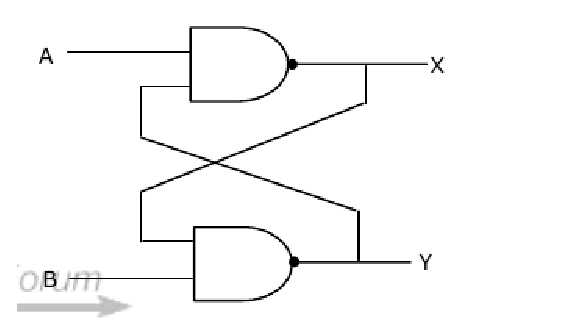
\includegraphics[width=\columnwidth]{./figs/6.eps}

\caption{}

\label{fig:6}

\end{figure} 


\begin{enumerate}[(a)]

\item fixed at $0$ and $1$, respectively

\item $x=1010....$ while $y=0101....$

\item $x=1010....$ and $y=0101....$

\item fixed at $1$ and $0$, respectively


\end{enumerate}


\item An equivalent $2$'s complement representation of the $2$'s complement number $1101$ is

\begin{enumerate}[(a)]

\item $110100
$

\item $
001101
$

\item $
110111
$

\item $
111101
$

\end{enumerate}

\item Two $2$'s complement number having sign bits $x$ and $y$ are added and the sign bit of the result is $z$. Then, the occurrence of overflow is indicated by the Boolean function

\begin{enumerate}[(a)]

\item $ x \ y \ z $

\item $ \overline{x} \ \overline{y} \ \overline{z} $

\item $ \overline{x} \ \overline{y} \ z \ + \ x \ y \ \overline{z}$

\item $ xy \ + \ yz \ + \ zx $

\end{enumerate}


\item Fig. \ref{fig:7}, shows a $mod-K$ counter, here $K$ is equal to

\begin{figure}

\centering

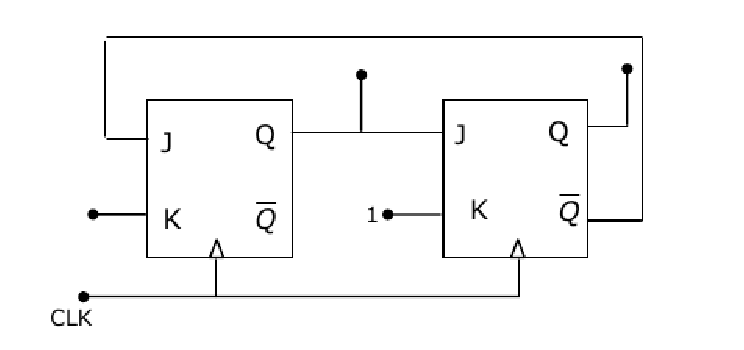
\includegraphics[width=\columnwidth]{./figs/7.eps}

\caption{}

\label{fig:7}

\end{figure} 


\begin{enumerate}[(a)]
 
\item $
1
$

\item $
2
$

\item $
3
$

\item $
4
$


\end{enumerate}

\item For a binary half-sub-tractor having two inputs $A$ and $B$, the correct set of logical expressions for the outputs $D$ (=$A$ minus $B$) and $X$(=borrow) are

\begin{enumerate}[(a)]
 
\item $
D = AB \ + \overline{A}B, X  =  \overline{A}B 
$

\item $
D = \overline{A}B \ +  A\overline{B} \ +  A \overline{B}, X  =  A\overline{B} 
$

\item $
D = \overline{A}B \ +  A \overline{B}, X  =  \overline{A}B 
$

\item $
D = AB \ +  \overline{A} \overline{B}, X  =  A \overline{B} 
$


\end{enumerate}

\item The ripple counter shown in Fig. \ref{fig:8} works as a

\begin{figure}

\centering

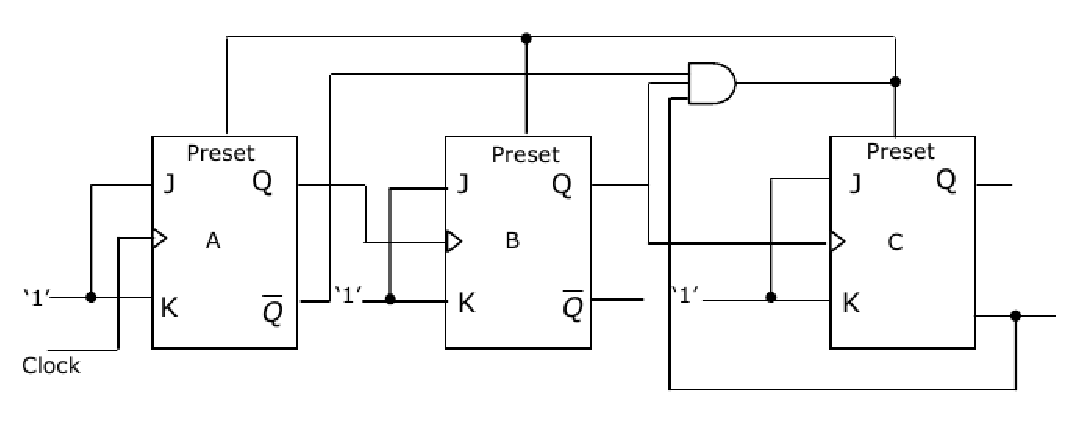
\includegraphics[width=\columnwidth]{./figs/10.eps}

\caption{}

\label{fig:8}

\end{figure} 



\begin{enumerate}[(a)]
 
\item mod - $3$ up counter

\item mod - $5$ up counter

\item mod - $3$ down counter

\item mod - $5$ down counter

\end{enumerate}

\item The circuit diagram of a synchronous counter is shown in Fig. \ref{fig:9}. Determine the sequence of states of the counter assuming that the initial state is $'000'$. Give your answer in a tabulor form showing the present state $Q_{A(n)},Q_{B(n)},Q_{C(n)},J-K$ inputs $(J_A,K_A,J_B,J_C,K)$ and the next state $Q_{A(n+1)},Q_{B(n+1)},Q_{C(n+1)}$. From the table, determine the modulus of the counter.

\begin{figure}

\centering

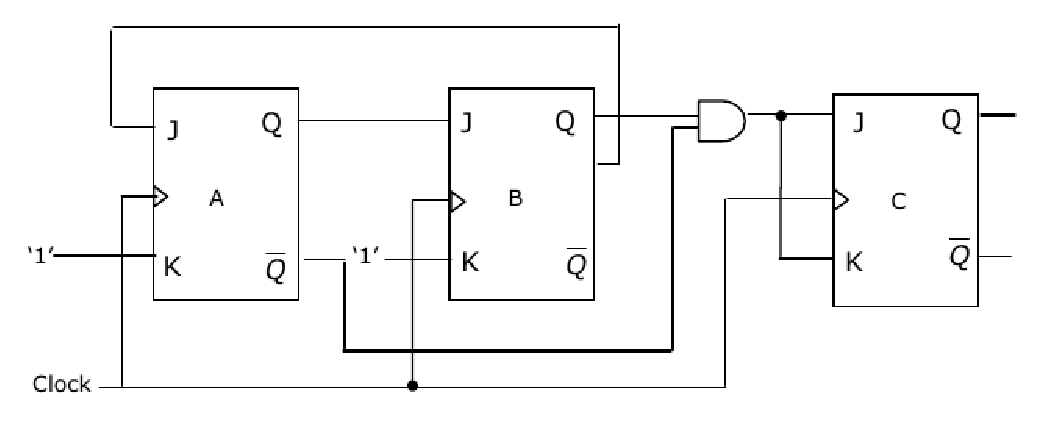
\includegraphics[width=\columnwidth]{./figs/11.eps}

\caption{}

\label{fig:9}

\end{figure} 



\item A sequential circuit using $D$ flip flop and logic gates is shown in Fig. \ref{fig:10},where $X$ and $Y$ are the inputs and $Z$ is the output. The circuit is

\begin{figure}

\centering

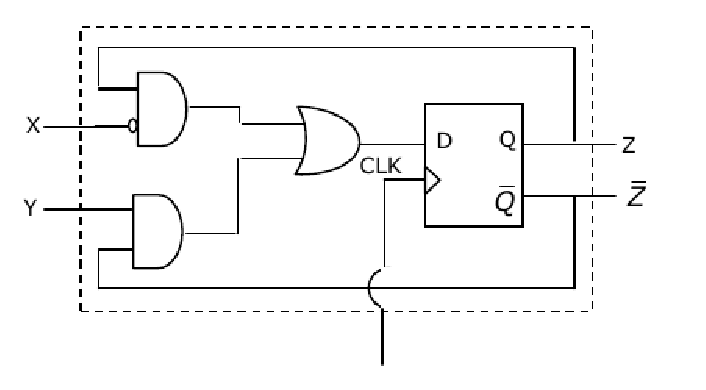
\includegraphics[width=\columnwidth]{./figs/12.eps}

\caption{}

\label{fig:10}

\end{figure} 




\begin{enumerate}[(a)]
 
\item $S-R$ Flip-Flop with inputs $X=R$ and $Y=S$

\item $S-R$ Flip-Flop with inputs $X=S$ and $Y=R$

\item $J-K$ Flip-Flop with inputs $X=J$ and $Y=K$

\item $J-K$ Flip-Flop with inputs $X=K$ and $Y=J$


\end{enumerate}
 
\item In Fig. \ref{fig:11}, the $J$ and $K$ inputs of all the four Flip-Flops are made high. The frequency of the signal at output $Y$ is

\begin{figure}

\centering

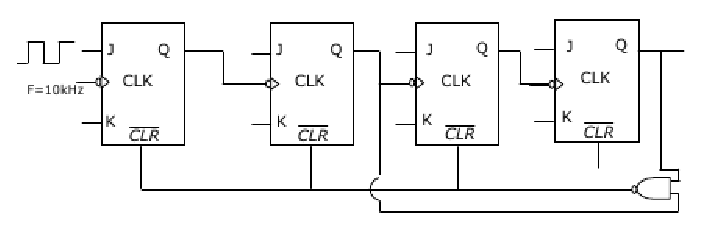
\includegraphics[width=\columnwidth]{./figs/15.eps}

\caption{}

\label{fig:11}

\end{figure} 



\begin{enumerate}[(a)]
 
\item $ 0.833 \ KHz$

\item $ 1.0 \ KHz$

\item $ 0.91 \ KHz$

\item $ 0.77 \ KHz$

\end{enumerate}



\item A one-bit full adder is to be implemented using $8$-to-$1$ multiplexers(MUX).

\begin{enumerate}[(a)]
 
\item Write the truth table for sum (S) and carry to the next stage $(C_N)$ in terms of the two bits$(A,B)$ and carry from the previous stage $(C_p)$.The truth table should be in the ascending order of $(A,B,C_p)$,i.e$(000,001,010,...$etc.).

\item Implement $S$ and $C_N$ using $8$-to-$1$ multiplexers.


\end{enumerate}


\item The voltage $e_0$ in Fig. \ref{fig:12} is


\begin{figure}

\centering

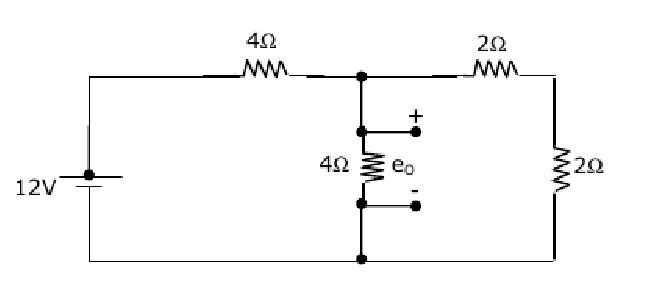
\includegraphics[width=\columnwidth]{./figs/16.eps}

\caption{}

\label{fig:12}

\end{figure} 


\begin{enumerate}[(a)]
 
\item $
2V
$

\item $
\frac{4}{3}V
$

\item $
4V
$

\item $
8V
$


\end{enumerate}

\item In the TTL circuit in Fig. \ref{fig:13}, $S_2$ to $S_0$ are select lines and $X_7$ and $X_0$ are input lines. $S_0$ and $X_0$ are LSBs. The output $Y$ is


\begin{figure}

\centering

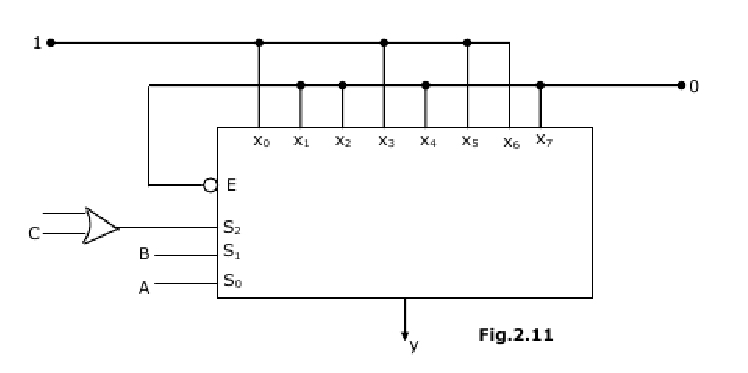
\includegraphics[width=\columnwidth]{./figs/17.eps}

\caption{}

\label{fig:13}

\end{figure} 



\begin{enumerate}[(a)]
 
\item indeterminate

\item $
A \ \oplus B
$

\item $
\overline{A \ \oplus B}
$

\item $
\overline{C}.(\overline{A \ \oplus B})+C.(A \ \oplus B)
$


\end{enumerate}


\item The digital block in Fig. \ref{fig:14} is realized using two positive edge triggered D-flip-flops. Assume that for $t < t_0$, $Q_1=Q_2=0$.The circuit in the digital block is given by:

\begin{figure}

\centering

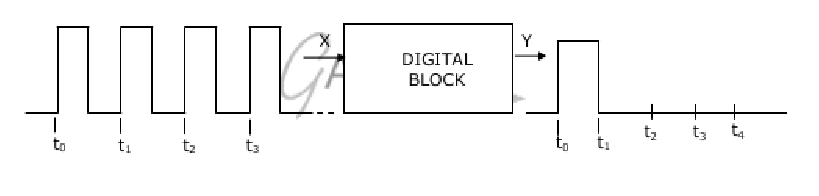
\includegraphics[width=\columnwidth]{./figs/18.eps}

\caption{}

\label{fig:14}

\end{figure} 


\begin{enumerate}[(a)]
 
\item Figure (a)

\item Figure (b)

\item Figure (c)

\item Figure (d)

\end{enumerate}

\begin{figure}

\centering

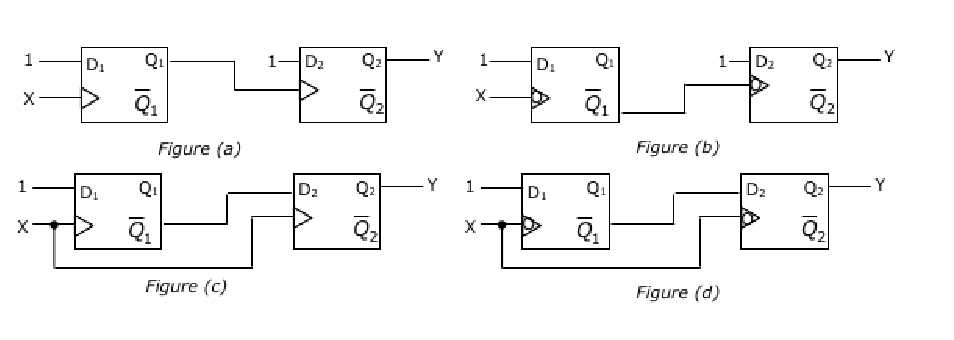
\includegraphics[width=\columnwidth]{./figs/19.eps}

\caption{}

\label{fig:15}

\end{figure} 


\item In Fig. \ref{fig:16}, the output of the oscillator, $V_1$ has $10V$ peak amplitude with zero $DC$ value. The transfer characteristic of the Schmitt inverter is also shown in Fig.  Assume that the $JK$ flip-flop is resent at time $t=0$.


\begin{figure}

\centering

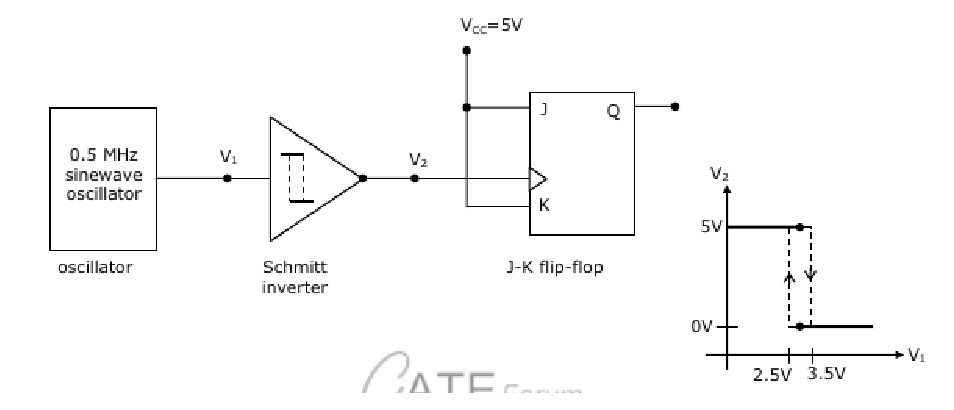
\includegraphics[width=\columnwidth]{./figs/20.eps}

\caption{}

\label{fig:16}

\end{figure} 


\begin{enumerate}[(a)]
 
\item What is the period and duty cycle of the waveform $V_2$?

\item What is the period and duty cycle of the waveform $V_3$?

\item Sketch $V_1,V_2 \ and \ V_3$ for the duration $0 \leq t \leq 6 \mu s.$ Clearly indicate the exact timings when the waveforms $V_2$ and $V_3$ make high-to-low and low-to-high transitions.

\end{enumerate}

\item In the network of Fig. \ref{fig:17}, the maximum power is delivered to $R_L$ if its value is 

\begin{figure}

\centering

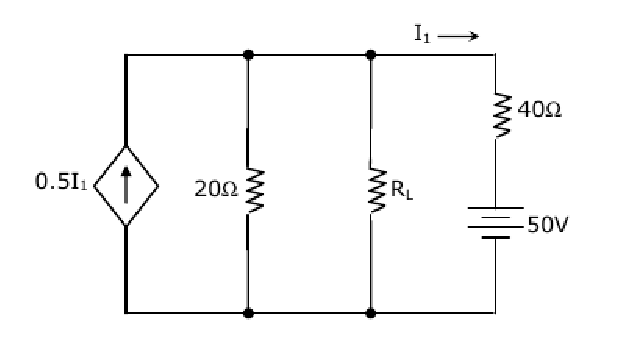
\includegraphics[width=\columnwidth]{./figs/21.eps}

\caption{}

\label{fig:17}

\end{figure} 



\begin{enumerate}[(a)]
 
\item $
16 \Omega $

\item $
\frac{40}{3} \Omega $


\item $
60 \Omega $

\item $
20 \Omega $


\end{enumerate}

\item If the input $X_3,X_2,X_1,X_0$ to the ROM in Fig. \ref{fig:18} are $8-4-2-1$ BCD numbers, then the outputs $Y_3,Y_2,Y_1,Y_0$ are

\begin{figure}

\centering

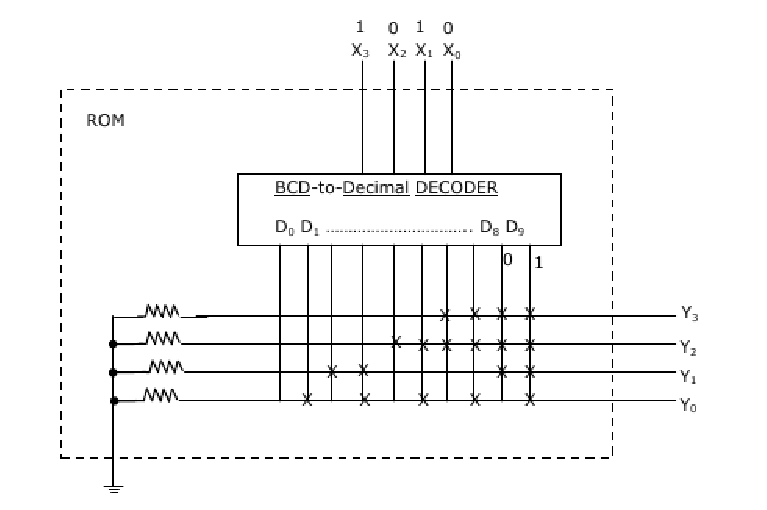
\includegraphics[width=\columnwidth]{./figs/22.eps}

\caption{}

\label{fig:18}

\end{figure} 



\begin{enumerate}[(a)]
 
\item gray code numbers

\item $2-4-2-1$ BCD numbers

\item excess $3$ code numbers

\item none of the above


\end{enumerate}


\item The inputs to a digital circuit shown in Fig. \ref{fig:19} are the external signals $A,B$ and $C$.

\begin{figure}

\centering

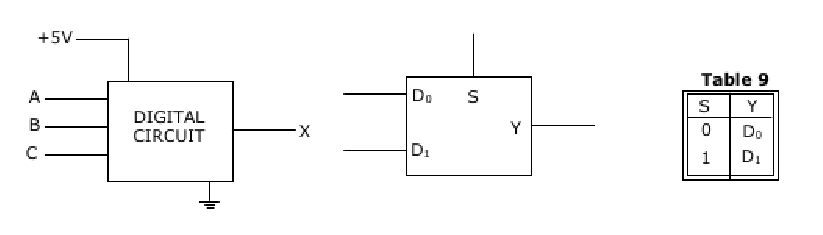
\includegraphics[width=\columnwidth]{./figs/23.eps}

\caption{}

\label{fig:19}

\end{figure} 


($\overline{A},\overline{B}$ and $\overline{C}$ are not available). The $+5V$ power supply (logic $1$ ) and the ground (logic $0$ ) are also available. The output of the circuit is $X=\overline{A}B+\overline{A}\ \overline{B} \ \overline{C}$.


\begin{enumerate}[(a)]
 
\item Write down the output function in its canonical SOP and POS forms.

\item Implement the circuit using only two $2:1$ multiplexers shown in figure (b),where S is the data-select line $D_0$ and $D_1$ are the input data lines and $Y$ is the output lines. The function table for the multiplexer is given in table $9$.

\end{enumerate}


\item It is required to design a binary mod-$5$ synchronous counter using AB flip-flops such that the output $Q_2,Q_1,Q_0$ changes as $ 000 \rightarrow 001 \rightarrow 010 .....$ and so on. The excitation table for the AB flip-flop is given in table.

\begin{enumerate}[(a)]
 
\item Write down the state table for the mod-$5$ counter.

\item Obtain simplified SOP expressions for the inputs $A_2,B_2,A_1,B_1,A_0$ and $B_0$ in terms of $Q_2,Q_1,Q_0$ and their complements.

\item Hence, complete the circuit diagram for the mod-$5$ counter given in Fig. \ref{fig:20} using minimum number of $2$-input NAND-gate only.


\begin{figure}

\centering

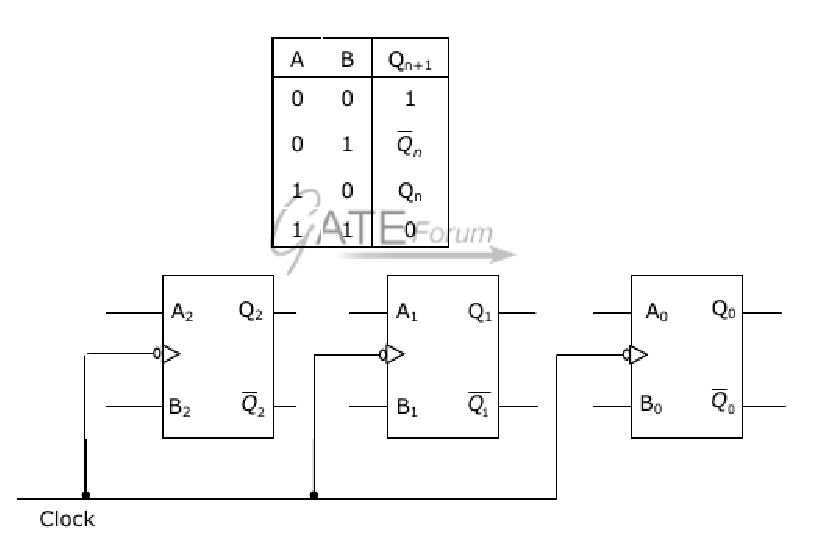
\includegraphics[width=\columnwidth]{./figs/24.eps}

\caption{}

\label{fig:20}

\end{figure} 




\end{enumerate}

\item Without any additional circuitry, an $8:1$ MUX can be used to obtain 


\begin{enumerate}[(a)]
 
\item some but not all Boolean functions of $3$ variables

\item all function of $3$ variables but none of $4$ variables

\item all functions of $3$ variables and some but not all of $4$ variables

\item all functions of $4$ variables

\end{enumerate}


\item A $0$ to $6$ counter consists of $3$ flip flops and a combination circuit of $2$ input gate(s). The combination circuit consists of

\begin{enumerate}[(a)]
 
\item one AND gate

\item one OR gate

\item one AND gate and one OR gate

\item two AND gates

\end{enumerate}

\item The circuit shown in Fig. \ref{fig:21} has $4$ boxes each described by inputs $P,Q,R$ and outputs $Y,Z$ with

\begin{figure}

\centering

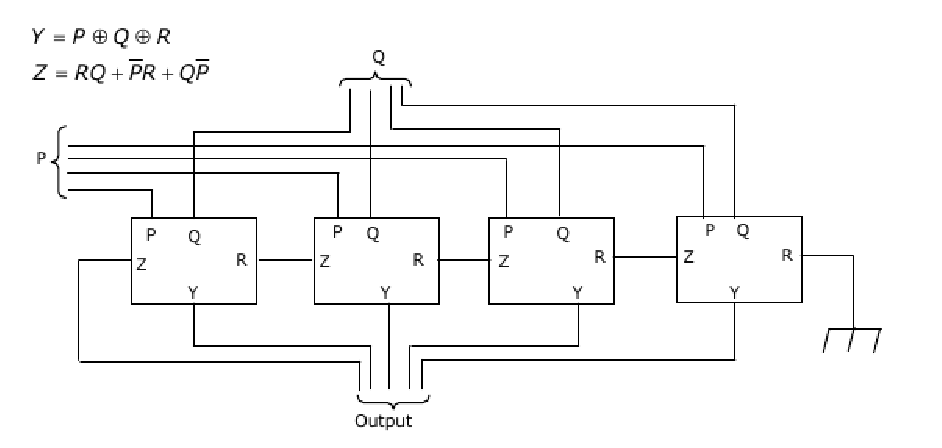
\includegraphics[width=\columnwidth]{./figs/25.eps}

\caption{}

\label{fig:21}

\end{figure} 


The circuit acts as a


\begin{enumerate}[(a)]
 
\item $4$ bit adder giving $ P+Q $

\item $4$ bit subtractor-giving $ P-Q $

\item $4$ bit subtractor-giving $ Q-P $

\item $4$ bit adder giving $ P+Q+R $


\end{enumerate}


\item A $4$ bit ripple counter and a $4$ bit synchronous counter are made using flip-flops having a propagation delay of $10$ ns each. If the worst case delay in the ripple counter and the synchronous counter be $R$ and $S$ respectively, then  

\begin{enumerate}[(a)]
 
\item $ R= \ 10 \ ns,S=\ 40 \ ns $

\item $ R= \ 40 \ ns,S=\ 10 \ ns $

\item $ R= \ 10 \ ns,S=\ 30 \ ns $

\item $ R= \ 30 \ ns,S=\ 10 \ ns $


\end{enumerate}

\item A master slave flip-flop has the characteristic that 

\begin{enumerate}[(a)]
 
\item change in the input immediately reflected in the output

\item change in the output occurs when the state of the master is affected

\item change in the output occurs when the state of the slave is affected

\item both the master and the slave states are affected at the same time
\end{enumerate}

\item The range of signed decimal numbers that can be represented by $6$-bite $1$'s complement number is

\begin{enumerate}[(a)]
 
\item $
-31$ \ to $+31
$


\item $
-63$ \ to $+64
$


\item $
-64$ \ to $+63
$


\item $
-32$ \ to $+31
$
\end{enumerate}


\item Choose the correct one from among the alternatives $A,B,C,D$ after matching an item from Group $1$ with the most appropriate item in Group $2$.

\begin{figure}

\centering

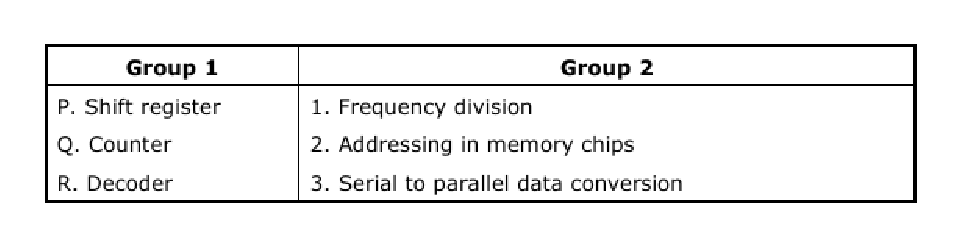
\includegraphics[width=\columnwidth]{./figs/26.eps}

\caption{}

\label{fig:22}

\end{figure} 


\begin{enumerate}[(a)]
 
\item $
P \ - 3 \ \ Q \ - 2 \ \ R - 1
$

\item $
P \ - 3 \ \ Q \ - 1 \ \ R - 2
$

\item $
P \ - 2 \ \ Q \ - 1 \ \ R - 3
$

\item $
P \ - 1 \ \ Q \ - 2 \ \ R - 2
$

\end{enumerate}

\item The minimum number of $2$ to $1$  multiplexers required to realize a $4$ to $1$ multiplexer is 

\begin{enumerate}[(a)]
 
\item $
1
$

\item $
2
$

\item $
3
$

\item $
4
$


\end{enumerate}

\item $11001,1001$ and $111001$ correspond to the $2$'s complement representation of which one of the following sets of number?

\begin{enumerate}[(a)]
 
\item $25,9$ and $57$ respectively

\item $-6,-6$ and $-6$ respectively

\item $-7,-7$ and $-7$ respectively

\item $-25,-9$ and $-57$ respectively

\end{enumerate}

\item In the modulo-$6$ ripple counter shown in Fig. \ref{fig:23}, the output of the $2$-input gate is used to clear the $J-K$ flip-flops.

\begin{figure}

\centering

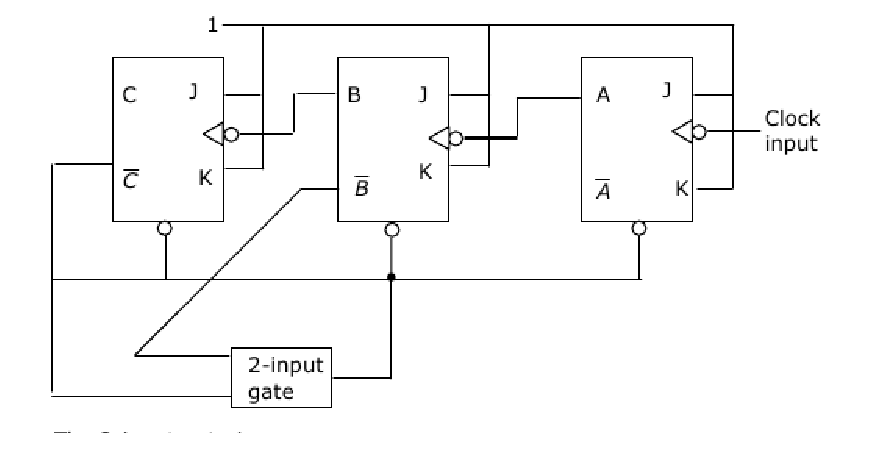
\includegraphics[width=\columnwidth]{./figs/27.eps}

\caption{}

\label{fig:23}

\end{figure} 




The $2$-input gate is 

\begin{enumerate}[(a)]
 
\item a NAND gate

\item a NOR gate

\item an OR gate

\item an AND gate

\end{enumerate}

\item The Boolean function $f$ implemented in Fig. \ref{fig:24} using two input multiplexers is 

\begin{figure}

\centering

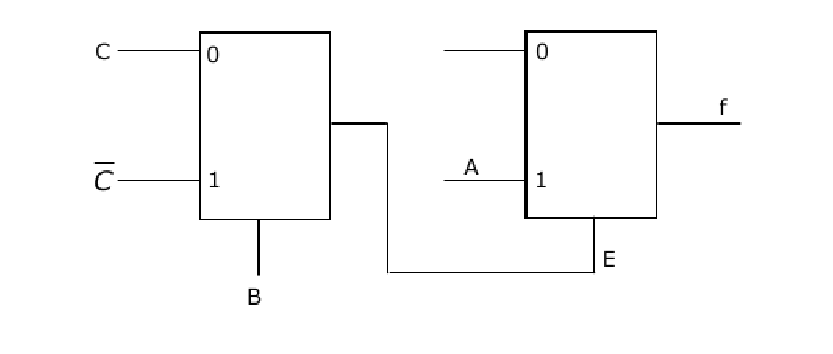
\includegraphics[width=\columnwidth]{./figs/28.eps}

\caption{}

\label{fig:24}

\end{figure} 



\begin{enumerate}[(a)]
 
\item $ A\overline{B}C \ + \ AB\overline{C} $

\item $ ABC \ + \ A\overline{B} \ \overline{C} $

\item $ \overline{A}BC \ + \ \overline{A} \ \overline{B} \ \overline{C} $

\item $ \overline{A} \ \overline{B}C \ + \ \overline{A}B\overline{C} $

\end{enumerate}

\item The present output $Q_n$ of an edge triggered $JK$ flip-flop is logic $0$. If $J=1$, then $Q_{n+1}$

\begin{enumerate}[(a)]
 
\item cannot be determined

\item will be logic $0$

\item will be logic $1$

\item will race around

\end{enumerate}


\item Fig.  \ref{fig:25} shows a ripple counter using positive edge triggered flip-flops. If the present state of counter is $Q_2Q_1Q_0=011$, then its next state $(Q_2Q_1Q_0)$ will be


\begin{figure}

\centering

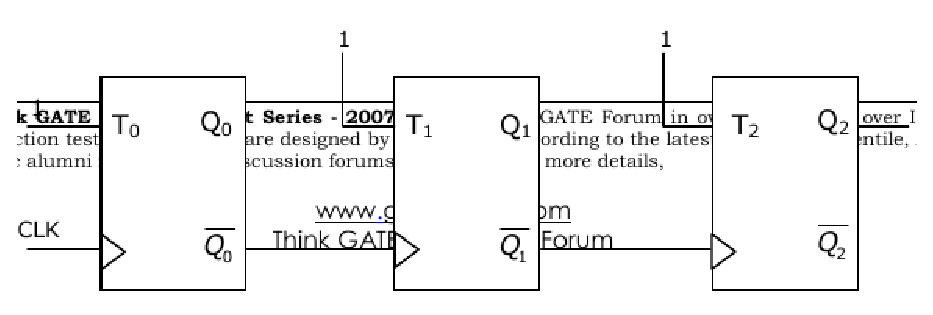
\includegraphics[width=\columnwidth]{./figs/29.eps}

\caption{}

\label{fig:25}

\end{figure} 



\begin{enumerate}[(a)]
 
\item $
010
$

\item $
100
$

\item $
111
$

\item $
101
$


\end{enumerate}


\item For the circuit shown in Fig. \ref{fig:26} below, two $4$-bit parallel-in serial-out shift registers loaded with the data shown are used to feed the data to a full adder. Initially, all the flip-flops are in clear state. After applying two clock pulses, the outputs of the full-adder should be

\begin{figure}

\centering

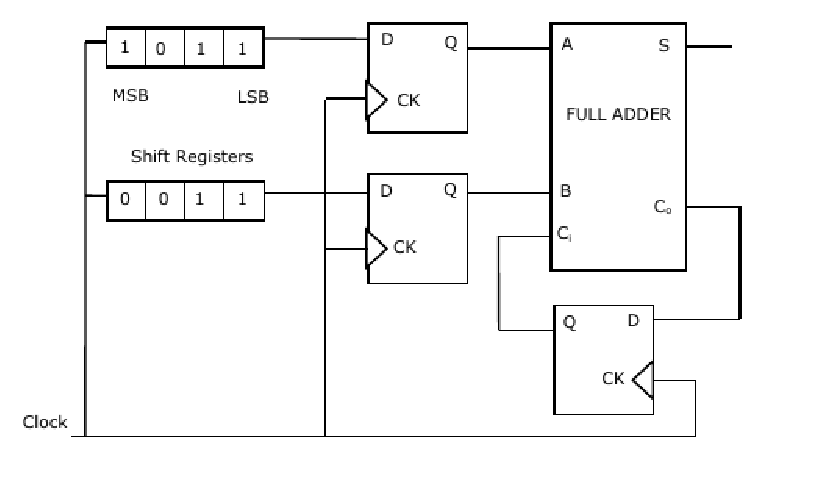
\includegraphics[width=\columnwidth]{./figs/30.eps}

\caption{}

\label{fig:26}

\end{figure} 



\begin{enumerate}[(a)]


\item $
S \ =0 \ \ C_0 \ = 0
$

\item $
S \ =0 \ \ C_0 \ = 1
$

\item $
S \ =1 \ \ C_0 \ = 0
$

\item $
S \ =1 \ \ C_0 \ = 1
$
\end{enumerate}

\item Two $D$-flip-flops, as shown below in Fig. \ref{fig:27}, are to be connected as a synchronous counter that goes through the following $Q_1Q_0$ sequence

$00 \rightarrow 01 \rightarrow 11 \rightarrow 10 \rightarrow 00 \rightarrow ...... $

The inputs $D_0$ and $D_1$ respectively should be connected as

\begin{figure}

\centering

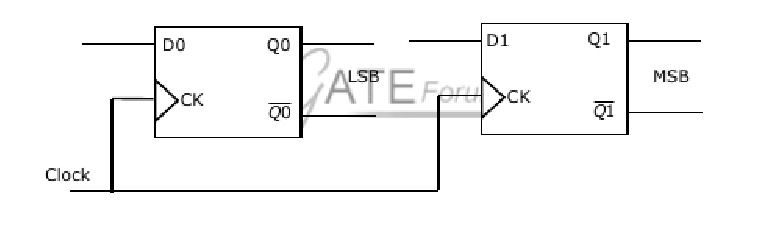
\includegraphics[width=\columnwidth]{./figs/31.eps}

\caption{}

\label{fig:27}

\end{figure} 


\begin{enumerate}[(a)]
 
\item $
\overline{Q_1}$ and $Q_0
$

\item $
\overline{Q_0}$ and $Q_1
$

\item $
\overline{Q_1}Q_0$ and $\overline{Q_1}Q_0
$

\item $
\overline{Q_1} \ \overline{Q_0}$ and $Q_1Q_0
$


\end{enumerate}

\item The point $P$ in the following Fig. \ref{fig:28} is stuck-at-$1$. The output $f$ will be 

\begin{figure}

\centering

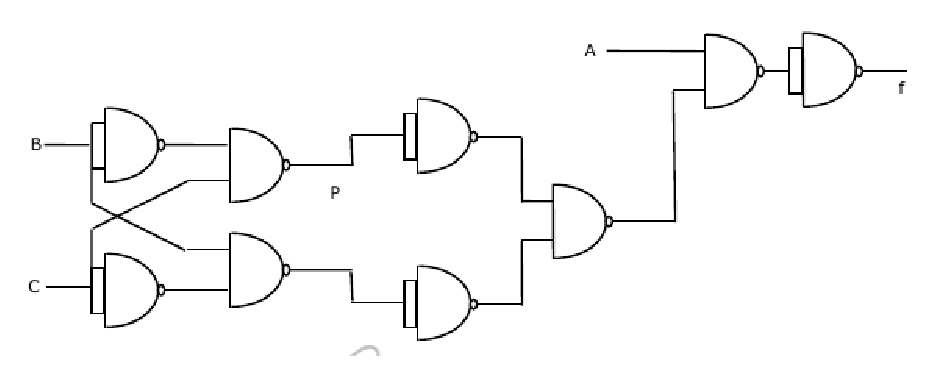
\includegraphics[width=\columnwidth]{./figs/32.eps}

\caption{}

\label{fig:28}

\end{figure} 



\begin{enumerate}[(a)]
 
\item $
\overline{AB\overline{C}}
$

\item $
\overline{A}
$

\item $
AB\overline{C}
$

\item $
A
$


\end{enumerate}

\item $X=01110$ and $Y=11001$ are two $5$-bit binary numbers represented in two's complement format. The sum of $X$ and $Y$ represented in two's complement format using $6$ bits is :


\begin{enumerate}[(a)]
 
\item $
100111
$

\item $
001000
$

\item $
000111
$

\item $
101001
$


\end{enumerate}
 
\item In the following circuit in Fig. \ref{fig:29}, $X$ is given by

\begin{figure}

\centering

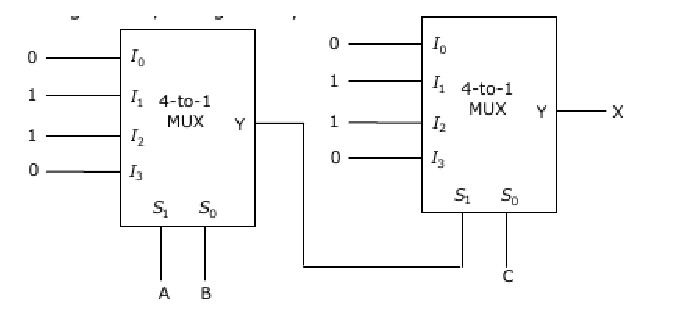
\includegraphics[width=\columnwidth]{./figs/34.eps}

\caption{}

\label{fig:29}

\end{figure} 

 
\begin{enumerate}[(a)]
 
\item $
X=\ A\overline{B} \ \overline{C} \ +\ \overline{A}B\overline{C} \ + \ \overline{A} \ \overline{B}C \ + \ ABC 
$

\item $
X=\ \overline{A}BC \ +\ A\overline{B}C \ + \ AB\overline{C} \ + \ \overline{A}\ \overline{B} \ \overline{C}
$

\item $
X= \ AB \ +\ BC \ + \ AC
$

\item $
X= \ \overline{A} \ \overline{B} \ +\ \overline{B} \ \overline{C} \ + \ \overline{A} \ \overline{C}
$


\end{enumerate}

\item The following binary values were applied to the $X$ and $Y$ inputs of the NAND latch shown in the Fig. \ref{fig:30} in the sequence indicated below:

$ X=0,Y=1$; \ $ X=0,Y=0$; \ $ X=1,Y=1$; \

The corresponding stable $P$,$Q$ outputs will be : 


\begin{figure}

\centering

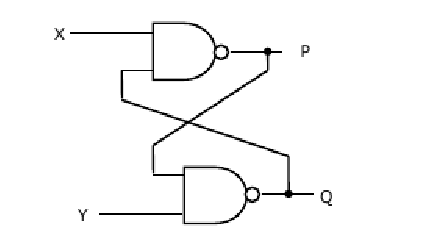
\includegraphics[width=\columnwidth]{./figs/35.eps}

\caption{}

\label{fig:30}

\end{figure} 

 

\begin{enumerate}[(a)]
 
\item $ P=1,\ Q=0$; \  $ P=1,\ Q=0$; \ \ \ \ \ \ \ $ P=1,\ Q=0$ or $ P=0,\ Q=1$

\item $ P=1,\ Q=0$; \  $ P=0,\ Q=1$; or $ P=0,\ Q=1$ \ \ \ \ \ \ \  $ P=0,\ Q=1$ 

\item $ P=1,\ Q=0$; \  $ P=1,\ Q=1$; \ \ \ \ \ \ \ $ P=1,\ Q=0$ or $ P=0,\ Q=1$

\item $ P=1,\ Q=0$; \  $ P=1,\ Q=1$; \ \ \ \ \ \ \ \ \ \ \ \ \ \ \ \ \ \ \ \ \ \ \ \ \ \ \ \ \ \ $ P=1,\ Q=1$ 


\end{enumerate}
 

\item For the circuit shown, the counter state $(Q_1Q_0)$ follows the sequence

\begin{figure}

\centering

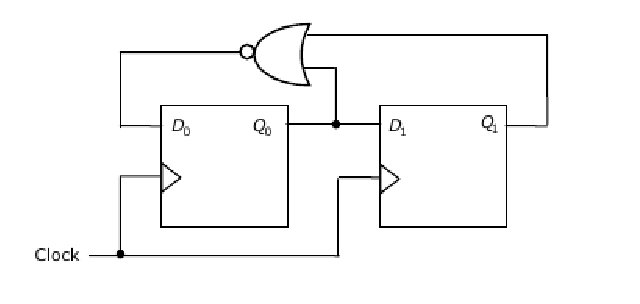
\includegraphics[width=\columnwidth]{./figs/36.eps}

\caption{}

\label{fig:31}

\end{figure} 




\begin{enumerate}[(a)]
 
\item $ 00,\ 01,\ 10,\ 11,\ 00 ... $

\item $ 00,\ 01,\ 10,\ 00,\ 01 ... $

\item $ 00,\ 01,\ 11,\ 00,\ 01 ... $

\item $ 00,\ 10,\ 11,\ 00,\ 10 ... $

\end{enumerate}
 
\item The two numbers represented in signed $2$'s complement form are $P=11101101$ and $Q=11100110$. If $Q$ is subtracted from $P$, the value obtained in signed $2$'s complement form is 

\begin{enumerate}[(a)]

\item $ 100000111 $

\item $ 00000111 $

\item $ 11111001 $

\item $ 111111001 $

\end{enumerate}

\item For the circuit shown in Fig. \ref{fig:32}, $32$ $I_0 - I_3$ are inputs to the $4:1$ multiplexer R(MSB) and $S$ are control bits

\begin{figure}

\centering

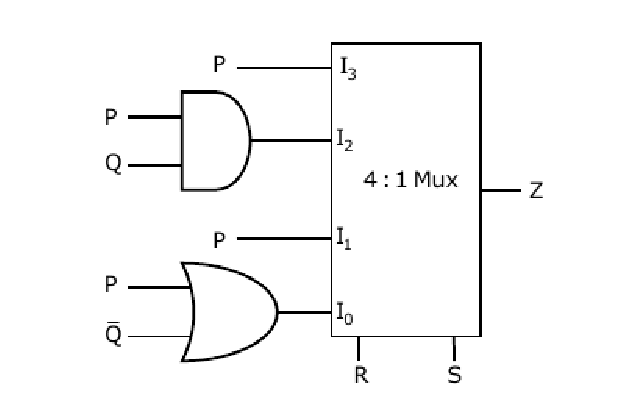
\includegraphics[width=\columnwidth]{./figs/37.eps}

\caption{}

\label{fig:32}

\end{figure} 


 
The output $Z$ can be represented by


\begin{enumerate}[(a)]

\item $ PQ+P\overline{Q}S+\overline{Q} \ \overline{R} \ \overline{S} $

\item $ P\overline{Q}+PQ\overline{R}+\overline{P} \ \overline{Q} \ \overline{S} $

\item $ P\overline{Q} \ \overline{R}+\overline{P}QR+PQRS+\overline{Q} \ \overline{R} \ \overline{S} $

\item $ PQ\overline{R}+PQR\overline{S}+P\overline{Q} \ \overline{R}S+\overline{Q} \ \overline{R} \ \overline{S} $

\end{enumerate}


\item For each of the positive edge-triggered $J-K$ flip flop used in the following Fig. \ref{fig:33},the propagation delay is $ \bigtriangleup T$

\begin{figure}

\centering

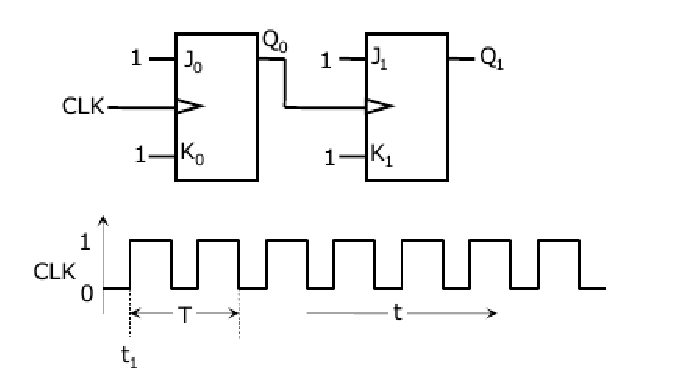
\includegraphics[width=\columnwidth]{./figs/38.eps}

\caption{}

\label{fig:33}

\end{figure} 
 


Which of the following waveforms in Fig. \ref{fig:34}  correctly represents the output at $Q_1$ ?

\begin{figure}

\centering

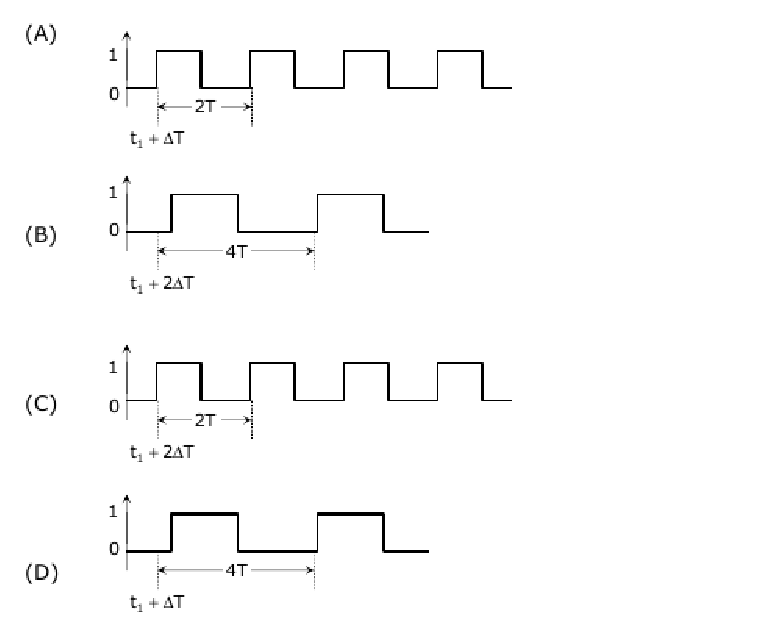
\includegraphics[width=\columnwidth]{./figs/39.eps}

\caption{}

\label{fig:34}

\end{figure} 


 
\item For the circuit shown in the Fig. \ref{fig:35}, $D$ has a transition from $0$ to $1$ after CLK changes from $1$ to $0$. Assume gate delays to be negligible

\begin{figure}

\centering

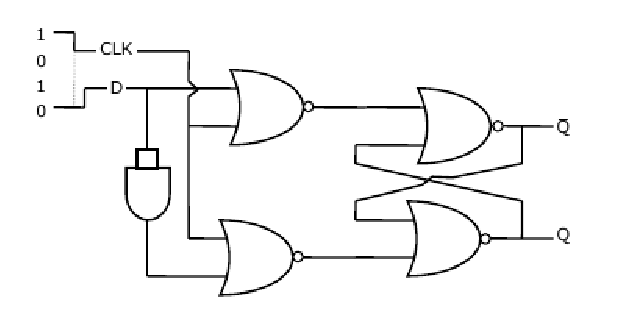
\includegraphics[width=\columnwidth]{./figs/40.eps}

\caption{}

\label{fig:35}

\end{figure} 


 
Which of the following statements is true?

\begin{enumerate}[(a)]

\item $Q$ goes to $1$ at the CLK transition and stays at $1$

\item $Q$ goes to $0$ at the CLK transition and stays at $0$

\item $Q$ goes to $1$ at the CLK transition and goes at $0$ when $D$ goes to $1$

\item $Q$ goes to $0$ at the CLK transition and goes to $1$ when $D$ goes to $1$

\end{enumerate}

\item The stable reading of the LED display is

\begin{enumerate}[(a)]

\item $ 06 $

\item  $ 07 $

\item $ 12 $

\item $ 13 $

\end{enumerate}

\item What are the minimum number of $2$-to-$1$ multiplexers required to generate a $2$-input AND gate and a $2$-input Ex-OR gate?

\begin{enumerate}[(a)]

\item $1$ and $2$

\item $1$ and $3$

\item $1$ and $1$

\item $2$ and $2$

\end{enumerate}

\item Refer to the NAND and NOR latches shown in the Fig. \ref{fig:36}. The inputs $(P_1,P_2)$ for both the latches are first made $(0,1)$ and then, after a few seconds, made $(1,1)$. The corresponding stable outputs $(Q_1,Q_2)$ are

\begin{figure}

\centering

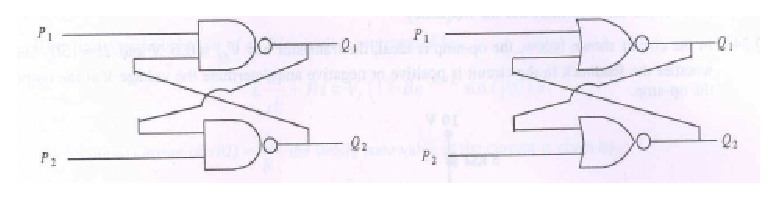
\includegraphics[width=\columnwidth]{./figs/41.eps}

\caption{}

\label{fig:36}

\end{figure} 

 
\begin{enumerate}[(a)]

\item NAND: first $(0,1)$ then $(0,1)$ \ \ NOR: first $(1,0)$ then $(0,0)$ 

\item NAND: first $(1,0)$ then $(1,0)$ \ \ NOR: first $(1,0)$ then $(1,0)$

\item NAND: first $(1,0)$ then $(1,0)$ \ \ NOR: first $(1,0)$ then $(0,0)$

\item NAND: first $(1,0)$ then $(1,1)$ \ \ NOR: first $(0,1)$ then $(0,1)$

\end{enumerate}

\item What are the counting states $(Q_1Q_2)$ for the counter shown in the Fig. \ref{fig:37} below?

\begin{figure}

\centering

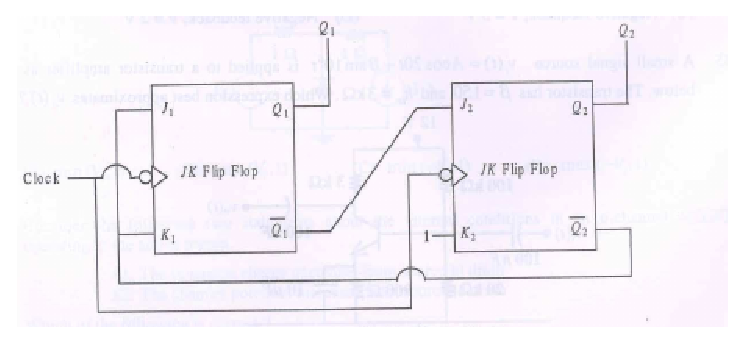
\includegraphics[width=\columnwidth]{./figs/42.eps}

\caption{}

\label{fig:37}

\end{figure} 


\begin{enumerate}[(a)]
 
\item $ 11,\ 10,\ 00,\ 11,\ 10 ... $

\item $ 01,\ 10,\ 11,\ 00,\ 01 ... $

\item $ 00,\ 11,\ 01,\ 10,\ 00 ... $

\item $ 01,\ 10,\ 00,\ 01,\ 10 ... $

\end{enumerate}
 
\item In the circuit shown, the device connected to $Y5$ can have address in the range


\begin{figure}

\centering

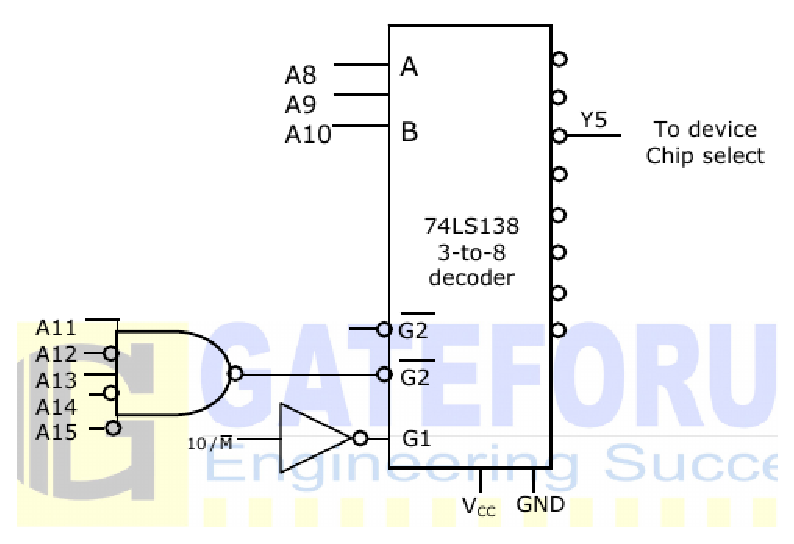
\includegraphics[width=\columnwidth]{./figs/43.eps}

\caption{}

\label{fig:38}

\end{figure} 



\begin{enumerate}[(a)]

\item $ 2000 - 20FF $

\item $ 2D00 - 2DFF $

\item $ 2E00 - 2EFF $

\item $ FD00 - FDFF $

\end{enumerate}

\item Assuming that flip-flops are in reset condition initially, the count sequence observed at $Q_A$ in the circuit shown is 

\begin{figure}

\centering

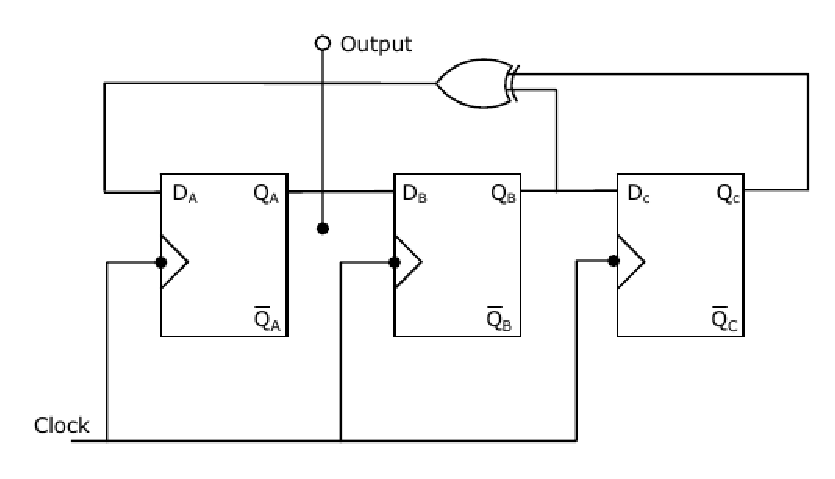
\includegraphics[width=\columnwidth]{./figs/44.eps}

\caption{}

\label{fig:39}

\end{figure} 




\begin{enumerate}[(a)]

\item $ 0010111... $

\item $ 0001011... $

\item $ 0101111... $

\item $ 0110100... $

\end{enumerate}

\item The Boolean function realized by the logic circuit shown is

\begin{figure}

\centering

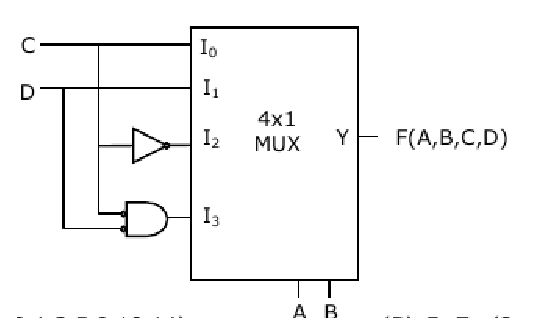
\includegraphics[width=\columnwidth]{./figs/46.eps}

\caption{}

\label{fig:40}

\end{figure} 



\begin{enumerate}[(a)]

\item $ F= \Sigma m (0,1,3,5,9,10,14) $

\item $ F= \Sigma m (2,3,5,7,8,12,13) $

\item $ F= \Sigma m (1,2,4,5,11,14,15) $

\item $ F= \Sigma m (2,3,5,7,8,9,12) $


\end{enumerate}

\item When the output $Y$ in the circuit below is $'1'$, it implies that data has 

\begin{figure}

\centering

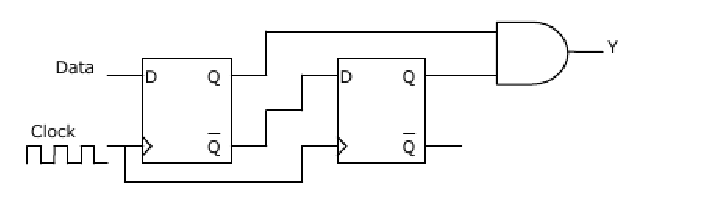
\includegraphics[width=\columnwidth]{./figs/47.eps}

\caption{}

\label{fig:41}

\end{figure} 


\begin{enumerate}[(a)]

\item changed from $0$ to $1$

\item changed from $1$ to $0$

\item changed in either direction

\item not changed 

\end{enumerate}

\item The logic function implemented by the circuit below is ( ground implies logic $0$ )

\begin{figure}

\centering

\includegraphics[width=\columnwidth]{./figs/48.eps}

\caption{}

\label{fig:42}

\end{figure} 



\begin{enumerate}[(a)]

\item $ F = AND(P,Q) $

\item $ F = OR(P,Q) $

\item $ F = XNOR(P,Q) $

\item $ F = XOR(P,Q) $

\end{enumerate}

\item The output of a $3$-stage Johnson (twisted ring) counter is fed to a digital-to-analog $(D/A)$ converter as shown in Fig.  \ref{fig:43}  below. Assume all the states of the counter to be unset initially. The waveform which represents the $D/A$ converter output $V_0$ is

\begin{figure}

\centering

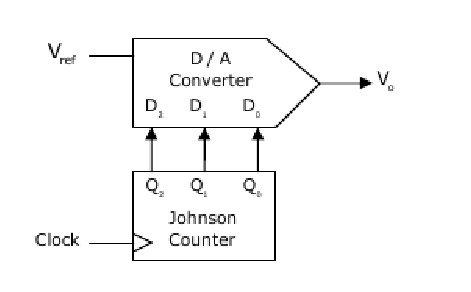
\includegraphics[width=\columnwidth]{./figs/49.eps}

\caption{}

\label{fig:43}

\end{figure} 

\begin{figure}

\centering

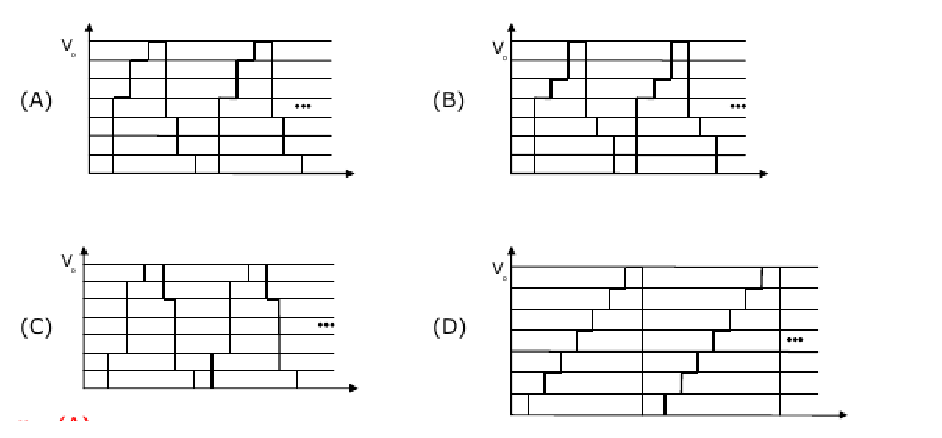
\includegraphics[width=\columnwidth]{./figs/50.eps}

\caption{}

\label{fig:44}

\end{figure} 



\item Two $D$ flip-flops are connected as a synchronous counter that goes through the following $Q_BQ_A$ sequence $ 00 \rightarrow 11 \rightarrow 01 \rightarrow 10 \rightarrow 00 \rightarrow ... $




The combination to the inputs $D_A$ and $D_B$ are

\begin{enumerate}[(a)]

\item $ D_A = Q_B ; D_B = Q_A $

\item $ D_A = \overline{Q_A} ; D_B = \overline{Q_B} $

\item $ D_A = (Q_A \overline{Q_B} + \overline{Q_A}Q_B) ; D_B = \overline{Q_A}$ 

\item $ D_A = (Q_A Q_B + \overline{Q_A Q_B}) ; D_B = \overline{Q_B}$

\end{enumerate}

\item The output $Y$ of a $2$-bit comparator is logic $1$ whenever the $2$-bit input $A$ is greater than the $2$-bit input $B$. The number of combinations for which the output is logic $1$, is 

\begin{enumerate}[(a)]

\item $ 4 $

\item $ 6 $

\item $ 8 $

\item $ 10 $

\end{enumerate}

\item Consider the given circuit in Fig.  \ref{fig:45}.

\begin{figure}

\centering

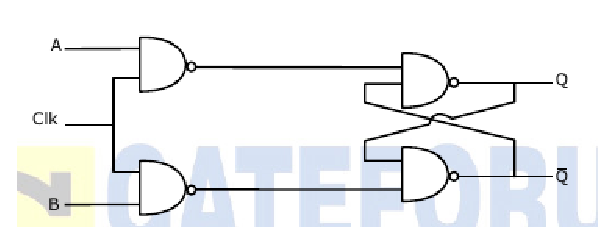
\includegraphics[width=\columnwidth]{./figs/51.eps}

\caption{}

\label{fig:45}

\end{figure} 



In this circuit, the race around

\begin{enumerate}[(a)]

\item does not occur

\item occurs when $CLK =0$

\item occur when $CLK = 1$ and $A = B = 1$ 

\item occurs when $CLK = 1$ and $A = B = 0$

\end{enumerate}

\item The state transition diagram for the logic circuit shown in Fig.  \ref{fig:46}  is 

\begin{figure}

\centering

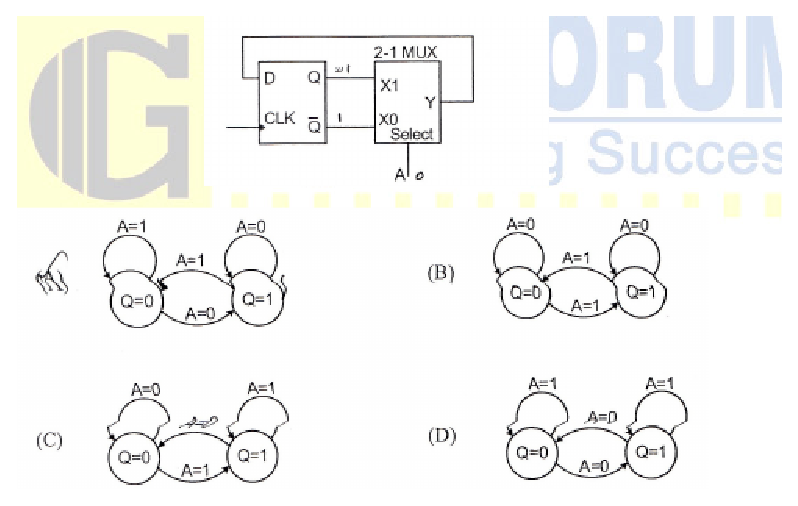
\includegraphics[width=\columnwidth]{./figs/52.eps}

\caption{}

\label{fig:46}

\end{figure} 




\item In the given circuit in Fig.  \ref{fig:47}, if $A$ is connected to $Q_1$, the operation of the circuit is according to the state diagram. If XOR is replaced with XNOR, then to get the same operation of the circuit which of the following changes has to be done

\begin{figure}

\centering

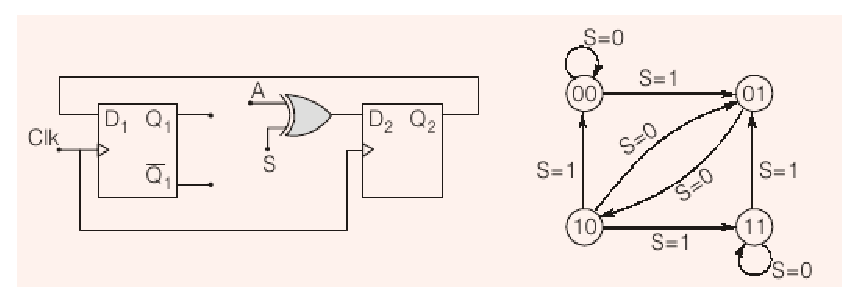
\includegraphics[width=\columnwidth]{./figs/53.eps}

\caption{}

\label{fig:47}

\end{figure} 



\begin{enumerate}[(a)]

\item $A$ should be connected to $\overline{Q_1}$

\item $A$ should be connected to $Q_2$

\item $A$ should be connected of $Q_1$ and $S$ is replaced  $\overline{S}$ to $ \overline{Q_1} $

\item $A$ should be connected to $\overline{Q_1}$ by $S$ is replaced by  $\overline{S} $

\end{enumerate}

\item The input frequency for the given counters $ 1 MHz$, the output frequency observes at $Q_4$ is $ \rule{3cm}{0.15mm}$


\begin{figure}

\centering

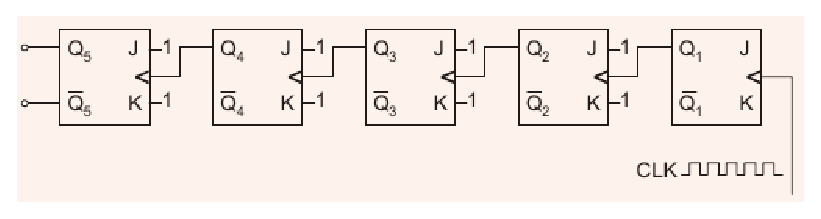
\includegraphics[width=\columnwidth]{./figs/54.eps}

\caption{}

\label{fig:48}

\end{figure} 


\item For the circuit given, if the clock frequency is $1 \ kHz$, then the frequency of output at $Q_3$ is $Hz$ $ \rule{3cm}{0.15mm}$


\begin{figure}

\centering

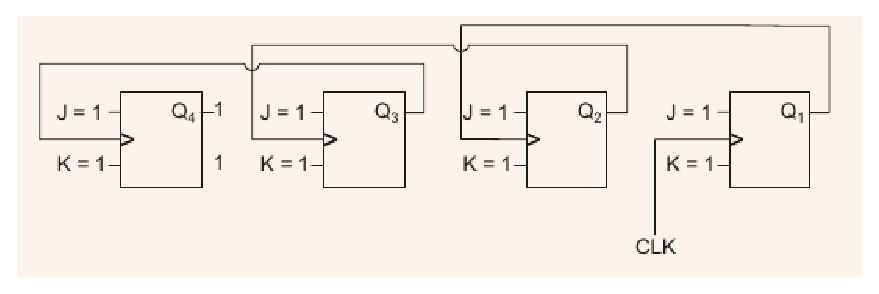
\includegraphics[width=\columnwidth]{./figs/55.eps}

\caption{}

\label{fig:49}

\end{figure} 


\item Consider the multiplexer based logic ckt. in Fig. \ref{fig:50} Find the boolean function = ?

\begin{figure}

\centering

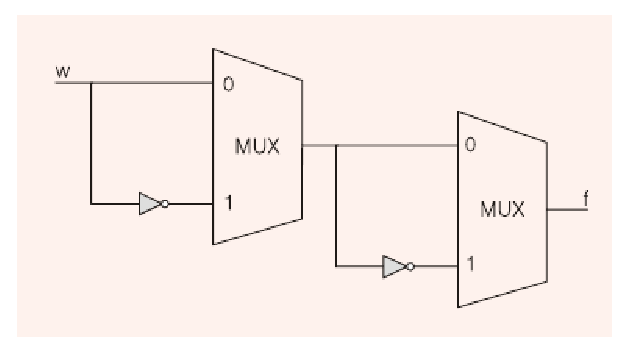
\includegraphics[width=\columnwidth]{./figs/56.eps}

\caption{}

\label{fig:50}

\end{figure} 



\begin{enumerate}[(a)]

\item $ f = w \overline{S_1} \ \overline{S_2} $

\item $ f = w S_1 + w S_2 + S_1 S_2 $

\item $ f = \overline{w} + S_1 + S_2 $

\item $ w \oplus S_1 \oplus S_2 $

\end{enumerate}


\item

 \begin{figure}

\centering

\includegraphics[width=\columnwidth]{./figs/57.eps}

\caption{}

\label{fig:51}

\end{figure} 



Current option is 

\begin{enumerate}[(a)]

\item $JK$ flip-flop

\item $SR$ flip-flop

\item $D$ flip-flop

\item Master-slave arrangement

\end{enumerate}

\item Find the output

\begin{figure}

\centering

\includegraphics[width=\columnwidth]{./figs/58.eps}

\caption{}

\label{fig:52}

\end{figure} 



y = $ \rule{3cm}{0.15mm}$

 
\begin{enumerate}[(a)]

\item $ w'x'y + wx'y $

\item $ wxy + wx'y' $

\item $ w'x'y' + xw'y + xyw $

\item none

\end{enumerate}

\item Assume that all the digital gates in the circuit shown in the Fig. \ref{fig:53} are ideal, the resistor $ R = 10 \ k\Omega $ and the supply voltage is $ 5 V $ .  The $D$ flip-flops $ D_1, D_2, D_3, D_4,$ and $D_5 $ are initialized with logic values $ 0,1,0,1 $ and $0$, respectively. The clock has a $ 30 \% $ duty cycle.

\begin{figure}

\centering

\includegraphics[width=\columnwidth]{./figs/59.eps}

\caption{}

\label{fig:53}

\end{figure} 



The average power dissipated ( in mW ) in the resistor $R$ is $ \rule{3cm}{0.15mm}$

\item The $ 4:1 $ multiplexer in Fig. \ref{fig:54} is to be used for generating the output carry of a full adder. $A$ and $B$ are the bits to be added while $ C_{in} $ is the input carry and $ C_{out} $ is the output carry. $A$ and $B$ are to be used as the select bits with $A$ being the more significant select bit.


\begin{figure}

\centering

\includegraphics[width=\columnwidth]{./figs/60.eps}

\caption{}

\label{fig:54}

\end{figure} 



Which one of the following statements correctly describes the choice of signals to be connected to the inputs $ I_0, I_1, I_2 $ and $ I_3 $ so that the output is $ C_{out}$ ?

\begin{enumerate}[(a)]

\item $ I_0=0, I_1=C_{in}, I_2=C_{in} $ and $ I_3=1 $

\item $ I_0=1, I_1=C_{in}, I_2=C_{in} $ and $ I_3=1 $

\item $ I_0=C_{in}, I_1=0, I_2=1 $ and $ I_3=C_{in} $

\item $ I_0=0, I_1=C_{in}, I_2=1 $ and $ I_3=C_{in} $

\end{enumerate}

\item The state transition diagram for a finite state machine with states $A,B$ and $C$, and binary inputs $X,Y$ and $Z$, is shown in Fig. \ref{fig:55}.


\begin{figure}

\centering

\includegraphics[width=\columnwidth]{./figs/61.eps}

\caption{}

\label{fig:55}

\end{figure} 




Which one of the following statements is correct?

\begin{enumerate}[(a)]

\item Transitions from State $A$ are ambiguously defined.

\item Transitions from State $B$ are ambiguously defined.

\item Transitions from State $C$ are ambiguously defined.

\item All of the state transitions are defined unambiguously.

\end{enumerate}

\item Consider the circuit shown in the Fig. \ref{fig:56}.

\begin{figure}

\centering

\includegraphics[width=\columnwidth]{./figs/62.eps}

\caption{}

\label{fig:56}

\end{figure} 



The Boolean expression $F$ implemented by the circuit is 

\begin{enumerate}[(a)]

\item $ \overline{X} \ \overline{Y} \ \overline{Z} + X \ Y + \overline{Y} \ Z $

\item $ \overline{X} \ Y \ \overline{Z} + X \ Z + \overline{Y} \ Z $

\item $ \overline{X} \ Y \ \overline{Z} + X \ Y + \overline{Y} \ Z $

\item $ \overline{X} \ \overline{Y} \ \overline{Z} + X \ Z + \overline{Y} \ Z $

\end{enumerate}


\item The state diagram of a finite state machine (FSM) designed to detect an overlapping sequence of three bits is shown in the Fig. \ref{fig:57}. The FSM has an input 'In' and an 'Out'. The initial state of the FSM is $ S_0$.

\begin{figure}

\centering

\includegraphics[width=\columnwidth]{./figs/63.eps}

\caption{}

\label{fig:57}

\end{figure} 


If the input sequence is $ 10101101001101 $, starting with the left-most bit, then the number of times 'Out' will be $1$ is $ \rule{3cm}{0.15mm}$ 

\item In Fig. \ref{fig:58},  Figure I shows a $4$-bit ripple carry adder realized using full adders and Figure II shows the circuit of a full-adder(FA). The propagation delay of the XOR, AND and OR gates in Figure II are $20$ ns, $15$ ns and $10$ ns,respectively. Assume all the inputs to the $4$-bit adder are initially reset to $0$.

\begin{figure}

\centering

\includegraphics[width=\columnwidth]{./figs/65.eps}

\caption{}

\label{fig:58}

\end{figure} 



At $t=0$,the inputs to the $4$-bit adder are changed to $X_3X_2 X_1 X_0 = 1100 $, $ Y_3 Y_2 Y_1 Y_0 = 0100 $ and $Z_0=1 $. The output of the ripple carry adder will be stable at $ t(in \ ns) =  \rule{3cm}{0.15mm}$ 

\item A four-variable Boolean function is realized using $ 4 \times 1 $ multiplexers as shown in the Fig. \ref{fig:59}.

\begin{figure}

\centering

\includegraphics[width=\columnwidth]{./figs/67.eps}

\caption{}

\label{fig:59}

\end{figure} 



The minimized expression for $F(U,V,W,X)$ is 

\begin{enumerate}[(a)]

\item $ (UV+\overline{U} \ \overline{V})\overline{W} $

\item $ (UV+\overline{U} \ \overline{V})(\overline{W} \ \overline{X}+\overline{W}X) $

\item $ (U\overline{V}+\overline{U}V)\overline{W} $

\item $ (U\overline{V}+\overline{U}V)(\overline{W} \ \overline{X}+\overline{W}X) $

\end{enumerate}

\item In the circuit shown below, a positive edge-triggered $D$ Flip-Flop is used for sampling input data $ D_{in} $ using clock $CK$. The XOR gate outputs $3.3$ volts for logic HIGH and $0$ volts for logic LOW levels.The data bit and clock periods are equal and the value of $ \Delta T / T_{CK}=0.15$, where the parameters $ \Delta T $ and $T_{CK}$ are shown in the Fig. \ref{fig:60}. Assume that the Flip-Flop and the XOR gate are ideal.

\begin{figure}

\centering

\includegraphics[width=\columnwidth]{./figs/68.eps}

\caption{}

\label{fig:60}

\end{figure} 




If the probability of input data bit $ (D_{in}) $ transition in each clock period is $0.3$, the average value (in volts, accurate to two decimal places) of the voltage at node $X$, is $ \rule{3cm}{0.15mm}$ 












\end{enumerate}
\end{document}
